Introducing STM as a electronically sensitive method to investigate surfaces, the atomic force microscopy interacts in a different way with the sample.
To scan the surface of the sample, one uses an small tip (cantilever) to interact with it. Due to its small distance different kinds of forces occur. The force induced movement of the tip is then interpreted and information about the surface may be derived.
\subsection{Theory}
The layout of a typical \index{AFM} consists of the cantilever itself and some kind of tip-position measurement. Earlier are made of the position-sensitive detector (PSD) consisting of two closely spaced photo diodes whose output signal is collected by a differential amplifier. Todays AFMs feature a Q-Plus sensor, as shown in \autoref{fig:AFM-qplus}. Here the tip is positioned on top of an oscillating fork that is operated close to its resonance frequency. If the tip interacts with the sample, its oscillations is hindered and the frequency of the oscillation shifts. From this shift in frequency one can estimate the strength of the acting force. Since every type of adsorbate atom acts in different ways with the tip, AFM is element specific. A magnetic tip can be used to scan for magnetic forces on the sample surface. With an added wire to the AFM tip, simultaneous AFM and STM measurements are possible. 

\begin{figure}\centering
	\subfigure[Photograph of the tuning fork and cantilever. The tip is glued to the tuning fork on the left side. From \cite{he_bottom-up_2017}]{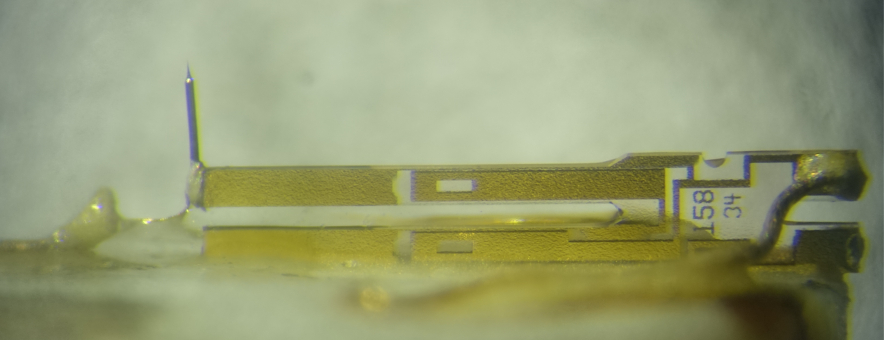
\includegraphics[width=0.6\textwidth]{./images/AFM-qplus-photograph}
		\label{fig:AFM-cantilever}}	
	\subfigure[QPlus sensor used to excite oscillations of the cantilever with controlled amplitude and frequency. Simultanious excitation of the tuning fork ($S_-$ and $S_+$) and measurement of the tunneling current ($I_t$) is possible. From \cite{AFM-qplus}]{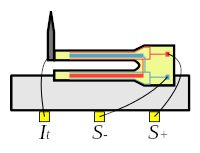
\includegraphics[width=0.3\textwidth]{./images/200px-QPlusSchematic}
		\label{fig:AFM-qplus}}
	
	\caption{Photograph \subref{fig:AFM-cantilever} and sketch \subref{fig:AFM-qplus} of AFM cantilever as used in the used setup. }
	\label{fig:AFM-tuning-fork}
\end{figure}	


\begin{figure}\centering
	\subfigure[Schematic representation of cantilever tip and atomically flat sample surface. The force between both $F_{TS}$ is indicated with an arrow. The attractive/repulsive force regimes are shown for variing tip-sample distances. From \cite{pavlicek_generation_2017}]{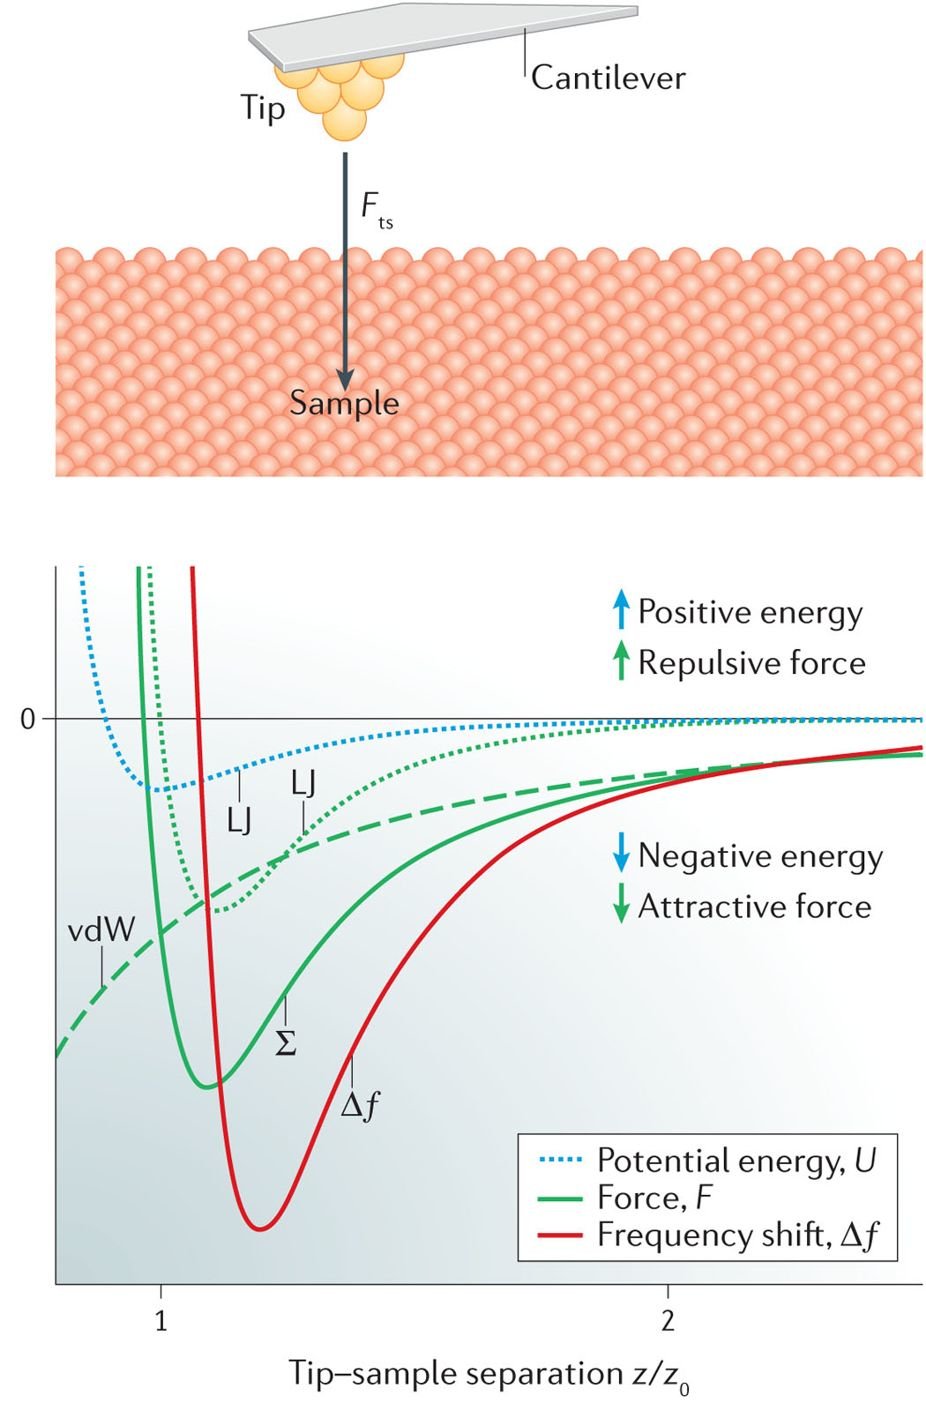
\includegraphics[width=0.6\textwidth]{./images/s41570-016-0005-f1}%
		\label{fig:AFM-force}}
	\subfigure[Enlarged sheme of AFM tip and top most sample layer with single adsorbate atom. CO functionalization of the tip leads to an decreased tip apex that increases resolution. Modified from\cite{AFM-qplus}.]{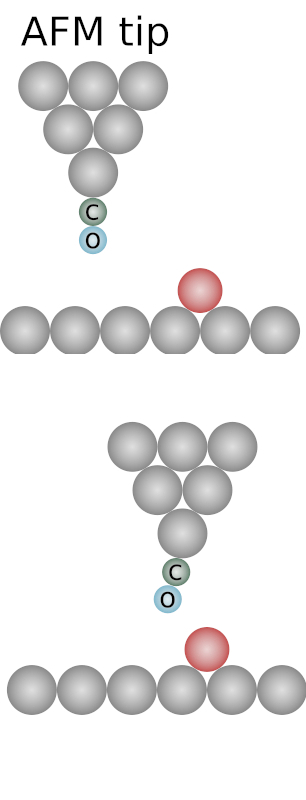
\includegraphics[width=0.3\textwidth]{./images/AFM_tip_with_CO-functionalization-mod}
		\label{fig:AFM-CO}}
	
	\caption{Basic function of a typical Q-plus AFM sensor. \subref{fig:AFM-force} Sketch of tip-sample interaction together with force-distance graph. The CO functionalization of the metalic AFM tip is shown in \subref{fig:AFM-CO}}%
	\label{fig:AFM-sketch}%
\end{figure}%
Types of forces are are typically:
\begin{itemize}
 \item Van-der-waals interaction (always attractive)
 \item Mechanical contact force (always repulsive)
 \item Capillary forces, chemical bonding, electrostatic forces, Casimir forces, solvation forces and others
\end{itemize}

The typical resulting force between tip and sample is artistically shown in \autoref{fig:AFM-force}. On the top part a cantilever with an atomic tip is shown on top of the sample surface. The interaction forces $F_{ts}$ act between tip and sample and are indicated by an arrow. In the lower part a representation of the resulting force in dependence of the tip-sample distance is shown. Although many different forces may act, the resulting potential is often modeled with a Lennard-Jones-Potential $LJ$\cite{jones_determination_1924}. Two of these are plotted with green and blue dots. The acting vdW force is plotted in dashed green. The sum of the acting forces is labeled $\sum$. A typical frequency shift $\Delta f$ is given as red graph. One can distinguish different regimes as indicated by the arrows. When tip and sample are in considerable distance to each other, the attractive vdW forces are the dominant part in the sum. While the tip approaches the sample, more and more interactions with the surface and adsorbate add to this force, strengthening $F_{ts}$. When the separation reaches $z_0$, the distance becomes so small that repulsive forces overcome the attractive one - entering the repulsive regime shortly afterwards. The best images were recorded close to the onset where $F_{ts}$ 

We used AFM in the nc-mode:
\begin{itemize}
  \item \textbf{Non-contact mode}: The cantilever is driven at its resonance frequency with amplitudes smaller than \SI{10}{\nm} and at a certain distance to the sample. Long-range forces like van-der-waals and others change the resonance frequency of the cantilever. This change is a indication of the acting force between cantilever and sample. This mode is used within the scope of this work.
\end{itemize}

\begin{itemize}
 \item AFM produces a true height-profile of the sample (and not a mix of electronic and geometric information projected onto a 2D-map like in STM)
 \item It has limited resolution especially when scanning features steeper than the tip apex
\end{itemize}

Its advantages are the comparable large image size of many hundred \si{\nm} compared to only some dozen \si{\nm} in the case of STM. Scan speeds are typically some orders of magnitude larger than those in STM so that image acquisition is much faster.

To increase the resolution the tip can be functionalized with CO (see figure \ref{fig:AFM-CO}). This method is widely used\footnote{Only a few examples from the recent years can be found here \cite{albrecht_direct_2016, kawai_multiple_2018, kawai_atomically_2015, schulz_elemental_2018, gross_chemical_2009, pavlicek_generation_2017, schwarz_corrugation_2017}} to investigate not only geometric features that are not accessible in STM, but also chemical differences on the sample\cite{wang_exploration_2017}.

\subsection{Experimental details}
\subsection{Methods}
\subsection{Limitations}